\documentclass[border=4pt,12pt]{standalone}
% House style for redrawn exam diagrams (diagram-v4: 0.4pt lines, filled -latex arrows, fine dashes; stipple and hatching drawn as real dots/lines (no PDF/SVG patterns, so they render in every browser and at any scale); transparent background). Every figure \input's this.
\usepackage{amsmath,amssymb}
\usepackage{txfonts}
\usepackage{pdfrender,xcolor}
% \halo{text}: label on shading. The shading stops just around each letter's outline (a thin knock-out that follows the
% glyphs, like the papers' typesetting), never a box. Owner: "I don't want a box around the text".
\newcommand{\halo}[1]{\leavevmode\rlap{\pdfrender{TextRenderingMode=2,LineWidth=2.2pt,LineJoinStyle=1,StrokeColor=white,FillColor=white}#1}#1}
\usepackage{tikz,pgfplots}
\pgfplotsset{compat=1.18}
\usetikzlibrary{arrows.meta,calc,angles,quotes,patterns,patterns.meta,intersections,positioning,decorations.markings,shapes.geometric}
% Stipple and hatching are drawn as actual dots / lines clipped to the region (path picture), NOT as pattern fills:
% SVG <pattern> fills vanish or blur when browsers scale the image, so the owner could not see the shading.
% Each dot is a 0.72pt square (keeps SVGs small; reads as a dot at print size). Dots sit on one global staggered grid, so neighbouring regions line up.
\makeatletter
\newdimen\ex@x \newdimen\ex@y \newdimen\ex@xa \newdimen\ex@ya \newdimen\ex@xb \newdimen\ex@yb \newcount\ex@row
\def\exam@stipplecolor{black!75}\def\exam@dotr{0.42pt}\def\exam@dotgap{2.5}
\def\ex@rowdots{\ifdim\ex@x<\ex@xb \pgfpathrectangle{\pgfqpoint{\dimexpr\ex@x-0.36pt\relax}{\dimexpr\ex@y-0.36pt\relax}}{\pgfqpoint{0.72pt}{0.72pt}}\advance\ex@x by \exam@dotgap pt\relax\expandafter\ex@rowdots\fi}
\def\exam@stipple{%
  \pgftransformreset% dots are sized in real points even inside scaled pictures
  \pgfpointanchor{path picture bounding box}{south west}\ex@xa=\pgf@x \ex@ya=\pgf@y
  \pgfpointanchor{path picture bounding box}{north east}\ex@xb=\pgf@x \ex@yb=\pgf@y
  \pgfsetfillcolor{\exam@stipplecolor}\pgfmathsetmacro\ex@h{\exam@dotgap/2}%
  \pgfmathtruncatemacro\ex@r{floor(\ex@ya/\ex@h)-1}\ex@row=\ex@r\relax
  \ex@y=\ex@r\dimexpr\ex@h pt\relax
  \loop\ifdim\ex@y<\ex@yb
    \pgfmathtruncatemacro\ex@c{floor(\ex@xa/\exam@dotgap)-1}\ex@x=\ex@c\dimexpr\exam@dotgap pt\relax
    \ifodd\ex@row \advance\ex@x by \ex@h pt\fi
    \ex@rowdots
    \advance\ex@y by \ex@h pt \advance\ex@row by 1
    \ifnum\numexpr\ex@row-(\ex@row/4)*4\relax=0 \pgfusepath{fill}\fi% flush every 4 rows: bounded TeX memory, few clip copies in the SVG
  \repeat\pgfusepath{fill}}
\newdimen\ex@d
\def\exam@hatch#1{% #1 = 1 for /, -1 for \ ; lines 45 degrees, 3pt apart
  \pgftransformreset
  \pgfpointanchor{path picture bounding box}{south west}\ex@xa=\pgf@x \ex@ya=\pgf@y
  \pgfpointanchor{path picture bounding box}{north east}\ex@xb=\pgf@x \ex@yb=\pgf@y
  \ex@d=\dimexpr\ex@yb-\ex@ya\relax \ex@x=\dimexpr\ex@xa-\ex@d\relax
  \loop\ifdim\ex@x<\ex@xb
    \ifnum#1>0 \pgfpathmoveto{\pgfqpoint{\ex@x}{\ex@ya}}\pgfpathlineto{\pgfqpoint{\dimexpr\ex@x+\ex@d\relax}{\ex@yb}}%
    \else \pgfpathmoveto{\pgfqpoint{\ex@x}{\ex@yb}}\pgfpathlineto{\pgfqpoint{\dimexpr\ex@x+\ex@d\relax}{\ex@ya}}\fi
    \advance\ex@x by 4.24pt
  \repeat
  \pgfsetlinewidth{0.4pt}\pgfsetstrokecolor{black}\pgfusepath{stroke}}
\def\examstipple{\exam@stipple}\def\examhatch{\exam@hatch}\def\examsetstipplecolor#1{\def\exam@stipplecolor{#1}}\def\examsetdotgap#1{\def\exam@dotgap{#1}}
\makeatother
% (legacy pattern kept for old files)
% staggered stipple like the NESA papers' dotted shading
\pgfdeclarepatternformonly{exam stipple}{\pgfpointorigin}{\pgfqpoint{2.2pt}{2.2pt}}{\pgfqpoint{2.2pt}{2.2pt}}{%
  \pgfpathcircle{\pgfqpoint{0.55pt}{0.55pt}}{0.42pt}\pgfpathcircle{\pgfqpoint{1.65pt}{1.65pt}}{0.42pt}\pgfusepath{fill}}
\tikzset{
  every picture/.style={line width=0.6pt, >={Latex[length=2mm,width=1.3mm]}},
  curve/.style={line width=0.6pt},
  open arrow/.style={-{Latex[length=2mm,width=1.3mm]}},  % owner: filled -latex heads everywhere, no open chevrons
  aux/.style={dash pattern=on 2pt off 1.5pt, line width=0.6pt},
  shade/.code={\def\exA{#1}\def\exB{none}\ifx\exA\exB\else\pgfkeysalso{fill=black!18}\fi},
  shade/.default=on,
  shade dots/.style={fill=none, path picture={\examstipple}},
  stipple color/.code={\examsetstipplecolor{#1}},
  stipple gap/.code={\examsetdotgap{#1}},
  shade dense dots/.style={fill=none, stipple gap=1.6, path picture={\examstipple}},
  shade hatch/.style={fill=none, path picture={\examhatch{1}}},
  shade hatch reverse/.style={fill=none, path picture={\examhatch{-1}}},
  shade solid/.style={fill=black},
  pt/.style={circle, fill, inner sep=1.1pt},
  open pt/.style={circle, draw, fill=white, inner sep=1.1pt},
}
\pgfplotsset{
  exam axes/.style={axis lines=middle, axis line style={->}, xlabel={$x$}, ylabel={$y$},
    xlabel style={anchor=west}, ylabel style={anchor=south}, tick label style={font=\small},
    every axis plot/.append style={line width=0.6pt, black}, samples=200, clip=false,
    enlargelimits=false, axis on top},
}

\begin{document}
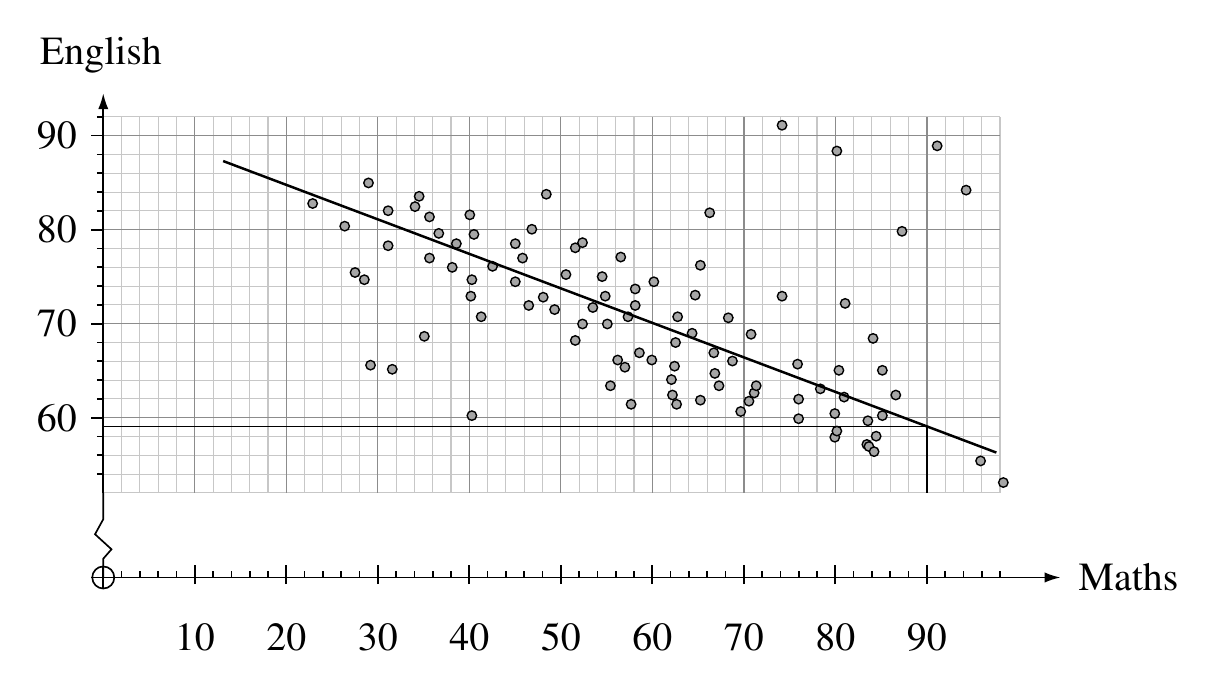
\begin{tikzpicture}[x=0.116205cm,y=0.11938cm]
\def\axE{43}
% grid
\foreach \m in {2,4,...,98} \draw[black!22,line width=0.4pt] (\m,52) -- (\m,92);
\foreach \e in {52,54,...,92} \draw[black!22,line width=0.4pt] (0,\e) -- (98,\e);
\foreach \m in {10,20,...,90} \draw[black!45,line width=0.5pt] (\m,52) -- (\m,92);
\foreach \e in {60,70,80,90} \draw[black!45,line width=0.5pt] (0,\e) -- (98,\e);
% y axis with break
\draw[->] (0,52) -- (0,94.5);
\draw (0,52) -- (0,49.2) -- (-0.9,47.6) -- (0.9,46) -- (0,45) -- (0,\axE);
\foreach \e in {54,56,58,62,64,66,68,72,74,76,78,82,84,86,88,92} \draw (-0.7,\e) -- (0,\e);
\foreach \e in {60,70,80,90} {\draw (-1.3,\e) -- (0,\e);
  \node[font=\Large,anchor=east] at (-1.8,\e) {$\e$};}
\node[font=\Large,anchor=west] at (-8,98.6) {English};
% x axis
\draw[->] (0,\axE) -- (104.6,\axE);
\foreach \m in {2,4,...,98} \draw (\m,\axE) -- (\m,\axE+0.7);
\foreach \m in {10,20,...,90} {\draw (\m,\axE-0.7) -- (\m,\axE+1.3);
  \node[font=\Large] at (\m,\axE-6.4) {$\m$};}
\node[font=\Large,anchor=west] at (105.5,\axE) {Maths};
\node[circle,draw,minimum size=2.8mm,inner sep=0] (o) at (0,\axE) {};
\draw (o.north) -- (o.south) (o.west) -- (o.east);
% data
\foreach \px/\py in {292/184,323/206,333/251,342/258,346/164,348/341,365/191,365/225,369/345,391/187,395/177,400/313,405/197,405/237,414/213,427/246,431/223,444/195,448/214,446/258,445/274,455/294,446/390,466/245,488/223,495/237,488/260,501/283,504/209,515/275,518/175,526/287,537/253,546/227,553/222,546/317,553/301,563/285,572/255,575/274,577/301,580/361,587/336,590/236,594/343,597/294,600/379,604/283,604/267,608/329,622/260,620/336,639/355,640/370,642/342,643/319,645/294,644/379,659/310,662/273,667/244,667/375,676/193,680/329,681/349,685/361,694/295,698/337,706/386,716/311,714/376,719/368,721/361,746/108,746/274,761/340,762/374,762/393,783/364,799/133,797/388,797/411,799/405,801/346,807/281,806/372,829/395,828/418,830/420,834/315,835/425,837/410,843/346,843/390,856/370,862/211,896/128,924/171,938/434,960/455}
  \node[circle,draw,fill=black!35,minimum size=1.2mm,inner sep=0,line width=0.5pt] at ({(\px-89.5)/8.85},{60-(\py-392)/9.13}) {};
% line of best fit and reading at Maths = 90
\def\fit#1{87.3-0.367*(#1-13.1)}
\draw[line width=0.9pt] (13.1,{\fit{13.1}}) -- (97.6,{\fit{97.6}});
\draw (0,{\fit{90}}) -- (90,{\fit{90}}) -- (90,52);
\end{tikzpicture}
\end{document}